\def \eng #1{\foreignlanguage{english}{#1}}
\def \engtt #1{\eng{\texttt{\justify #1}}}

\textbf{Цель работы.}
%
\begin{enumerate}
	\item Знакомство с интерфейсом \eng{Centronix}.
    \item Применение интерфейса \eng{Centronix} для двустороннего обмена информацией и управления лабораторным макетом.
\end{enumerate}

\textbf{Аппаратура.} Лабораторный макет \enquote{набор лампочек и кнопочек}, источник питания, персональный компьютер.

\textbf{Содержание работы.} Реализация световых эффектов на лампочках лабораторного макета с использованием информации о состоянии тумблеров тумблерного регистра на передней панели прибора. Реализация световых эффектов: \begin{enumerate*}[label=(\asbuk*)]
    \item бегущий огонь,
    \item бегущая тень,
    \item накапливающееся включение,
    \item \enquote{включен переключатель~--- горит соответствующий светодиод}.
\end{enumerate*}

\section{Минимальные теоретические сведения}

\subsection{Описание интерфейса параллельного порта \eng{Centronix}}

Основным назначением интерфейса \eng{Centronix} (аналог — ИРПР-М) является подключение к компьютеру принтеров различных типов. Поэтому распределение контактов разъема, назначение сигналов, программные средства управления интерфейсом ориентированы именно на это использование. В то же время с помощью данного интерфейса можно подключать к компьютеру и другие внешние устройства, имеющие разъем \eng{Centronix}, а также специально разработанные относительно несложные устройства сопряжения, не предъявляющие жестких требований по скорости информационного обмена и длине линии связи.

Все сигналы интерфейса можно разделить на четыре группы:

\begin{enumerate}
    \item восьмиразрядная шина данных для записи из компьютера (сигналы \engtt{D0 \dots D7});
    \item четырехразрядная шина управления для записи из компьютера (сигналы \engtt{-STROBE}, \engtt{-AUTO FD}, \engtt{-INIT} и \engtt{-SLCT IN});
    \item пятиразрядная шина состояния для чтения в компьютер (сигналы \engtt{-ACK}, \engtt{BUSY}, \engtt{PE}, \engtt{SLCT} и \engtt{-ERROR});
    \item шина \enquote{земли}.
\end{enumerate}

Все сигналы программно доступны, что позволяет реализовать произвольные протоколы информационного обмена в рамках имеющегося их набора и быстродействия компьютера.

Простейший анализ набора сигналов позволяет выделить основную проблему, возникающую при сопряжении устройств с интерфейсом \eng{Centronix}. Поскольку шина данных является однонаправленной, что позволяет использовать ее только на вывод (речь идет о базовом интерфейсе \eng{Centronix}, однако разработаны также модификации параллельного порта с двунаправленной шиной данных), для ввода данных необходимо использовать сигналы из пятиразрядной шины состояния. Таким образом, если не предпринимать специальных шагов, разрядность информационного обмена по чтению ограничена пятью линиями.

Временная диаграмма цикла передачи данных представлена на \autoref{fig:time_diagram}. Перед началом цикла передачи данных компьютер должен убедиться, что сняты сигналы \engtt{BUSY} и \engtt{-ACK}. После этого выставляются данные, формируется строб, снимается строб, и снимаются данные. Принтер должен успеть принять данные с выбранным темпом. При получении строба принтер формирует сигнал \engtt{BUSY}, а после окончания обработки данных выставляет сигнал \engtt{-ACK}, снимает \engtt{BUSY} и снимает \engtt{-ACK}. Затем может начинаться новый цикл.
%
\begin{figure}[h]%
    \centering
    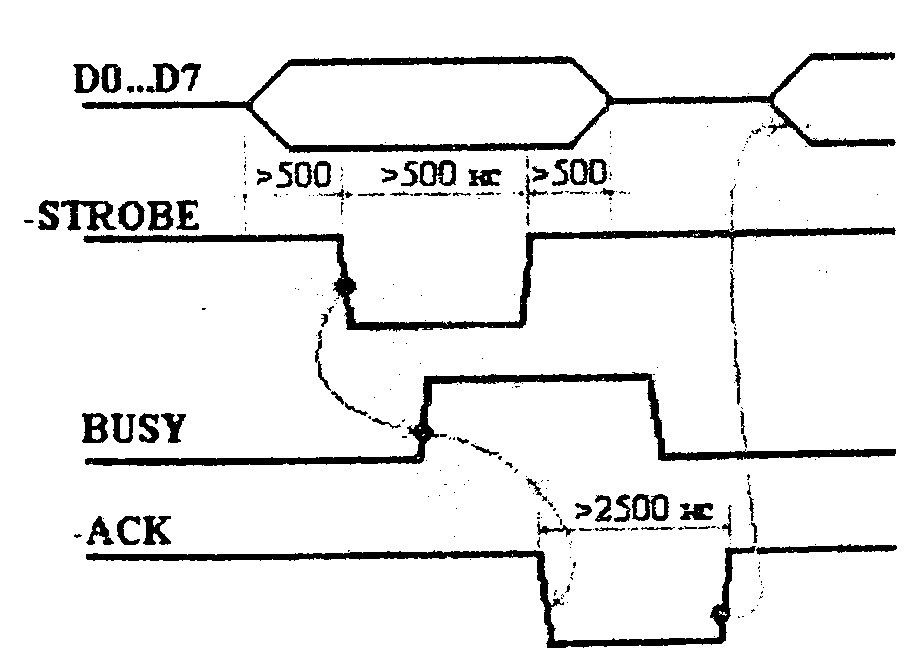
\includegraphics[width=0.5\textwidth]{time_diagram}%
    \caption[]{Временная диаграмма цикла передачи данных интерфейса \eng{Centronix}}%
    \label{fig:time_diagram}%
\end{figure}

При разработке нестандартных устройств для подключения к интерфейсу \eng{Centronix} его сигналы могут быть использованы произвольно по своему усмотрению.

Формирование и прием сигналов интерфейса \eng{Centronix} производится путем записи и чтения выделенных для него портов ввода/вывода. В компьютере может использоваться три порта \eng{Centronix} (обычно используется два порта), обозначаемых \eng{LPT1} (базовый адрес \eng{378h}), \eng{LPT2} (базовый адрес \eng{278h}) и \eng{LPT3} (базовый адрес \eng{3BCh}).

\subsection{Программирование интерфейса \eng{Centronix}}

Параллельный порт имеет три адреса в пространстве устройств ввода-вывода компьютера:

\begin{enumerate}
    \item \engtt{BASE}~--- регистр данных,
    \item \engtt{BASE+1}~--- регистр состояния,
    \item \engtt{BASE+2}~--- регистр управления,
\end{enumerate}

Здесь \engtt{BASE} — первый адрес порта. Таким образом, перед обращением к порту необходимо выполнить процедуру определения его базового адреса.

Программирование подключенной к параллельному порту аппаратуры заключается в установке определенных битов в регистрах данных и управления и чтении определенных битов из регистра состояния. При этом если с регистром данных проблем не возникает (это обычный байтовый регистр), то дня других регистра имеют некоторые особенности. Во-первых, некоторые биты являются инверсными. Во-вторых, если четыре бита регистра управления расположены в младших битах байта (биты 0-3), то пять битов регистра состояния~--- в старших (биты 3-7).

\subsection{Описание лабораторного макета}

Рассмотрим задачу управления устройством типа \enquote{набор лампочек и кнопочек}, содержащим переключатели и светодиоды, через интерфейс \eng{Centronix}. В зависимости от положения переключателей по некоторому алгоритму должны загораться светодиоды. Устройство должно подключаться к персональному компьютеру через параллельный порт.

На \autoref{fig:maket}-\autoref{fig:maket_scheme} показан вариант реализации такого устройства. Для управления светодиодами использованы сигналы \engtt{D0 \dots D7}, поэтому их число ограничено восемью. Триггеры К555ТМ8 объединены в составной регистр и предназначены для фиксации данных и начальной установки (гашения) светодиодов. Сигнал \engtt{-STROBE} используется для стробирования записи данных в регистр, а сигнал \engtt{-INIT}~--- для сброса регистра и гашения светодиодов (светодиод горит при записи логической \enquote{1} в соответствующий разряд регистра). При замыкании переключателя по соответствующей ему линии шины состояния читается логический \enquote{0}, а при размыкании логическая \enquote{1}.

Поскольку пяти линий шины состояния для ввода явно недостаточно для считывания состояний 8 переключателей, то в устройстве применен простой способ увеличения числа разрядов на ввод~--- мультиплексирование принимаемых данных. Мультиплексор КР555КП11 реализует преобразование восьми линий в четыре, которое выполняется в две фазы~--- ввод младшей тетрады и ввод старшей тетрады. Для переключения мультиплексора можно использовать свободный сигнал шины управления, например \engtt{-SLCT IN}.

\begin{figure}[h]%
    \centering
    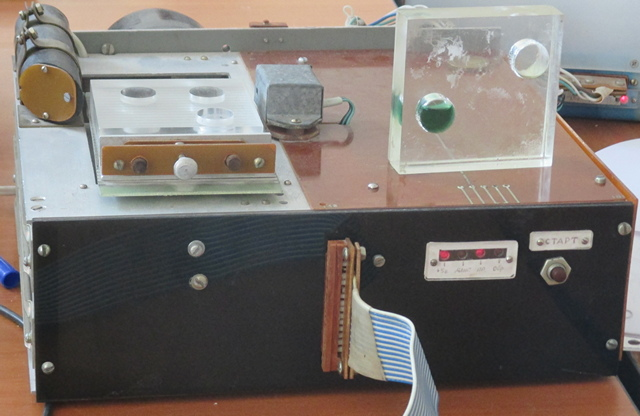
\includegraphics[width=0.8\textwidth]{maket}%
    \caption[]{Внешний вид лабораторного макета}%
    \label{fig:maket}%
\end{figure}
%
\begin{figure}[h]%
    \centering
    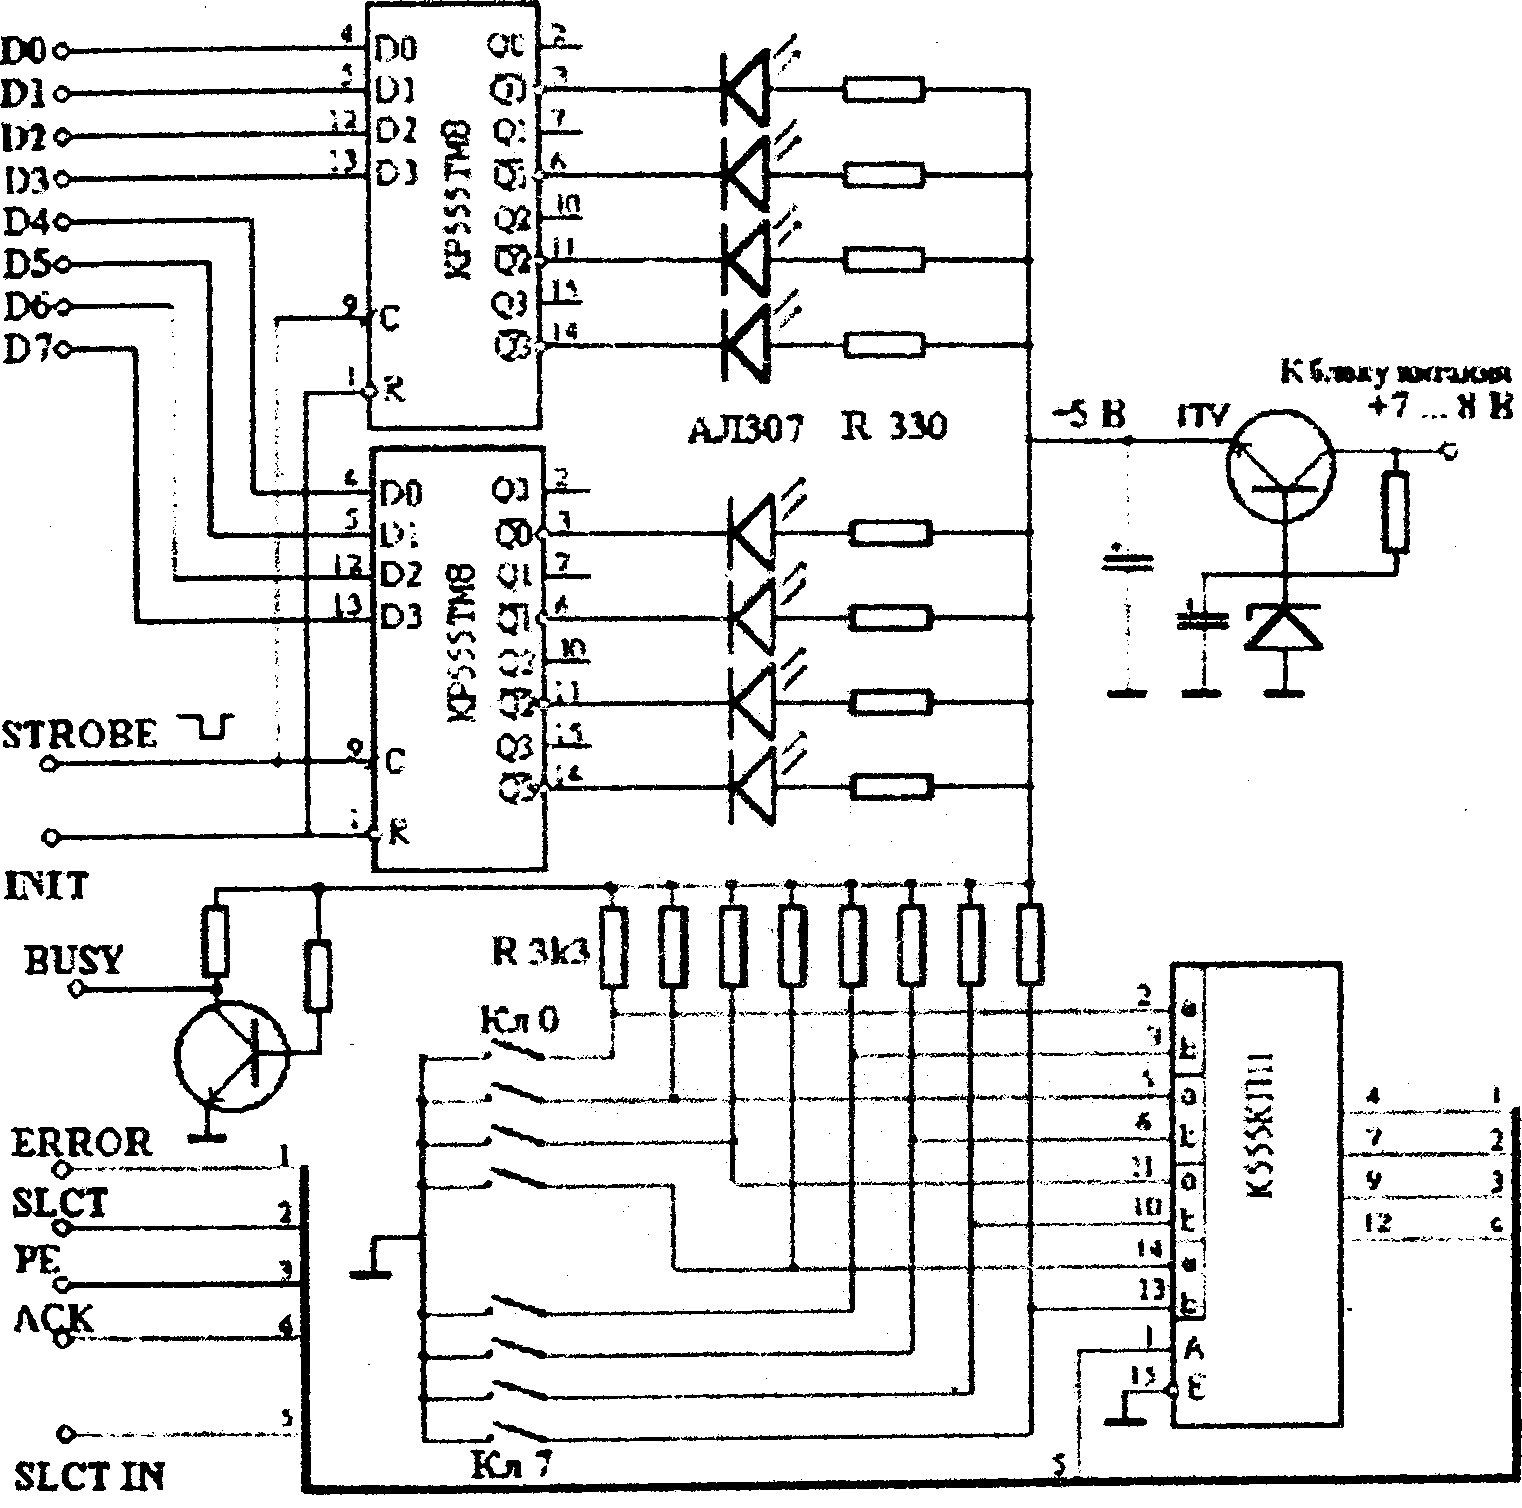
\includegraphics[width=0.5\textwidth]{maket_scheme}%
    \caption[]{Схема лабораторного макета}%
    \label{fig:maket_scheme}%
\end{figure}

\section{Результаты и их обсуждение}

\subsection{Интерфейс программы управления}

Для организации работы с устройством была разработана программа с графическим интерфейсом (\autoref{fig:app}).

\begin{figure}[h]%
\centering
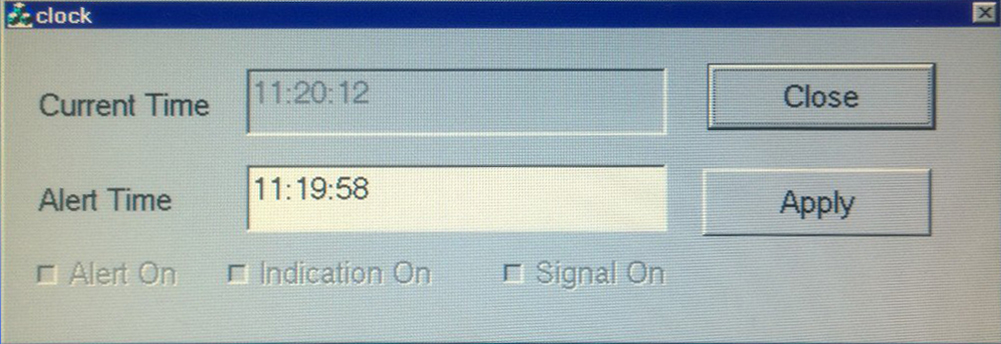
\includegraphics[width=0.5\textwidth]{app}%
\caption[]{Главное окно программы}%
\label{fig:app}%
\end{figure}

Программа в фоновом режиме следит за состоянием аппаратуры (наличие питания, состояние тумблерного регистра). При выборе соответствующего эффекта после изменения состояния тумблера изменяется и состояние расположенного над ним светодиода.

Операторский интерфейс программы предусматривает возможность выбрать тип светового эффекта и указать его параметры.

\subsection{Архитектура программы управления}

Программа управления была написана в среде \eng{Microsoft Visual Studio 6.0} на языке \engtt{c++} с использованием библиотеки классов \eng{MFC} (\eng{Microsoft Foundation Classes}).

Для инкапсуляции низкоуровневого программного интерфейса устройства был описан и реализован интерфейс (абстрактный класс) \engtt{CDevice}. Он инкапсулирует все этапы двустороннего обмена информацией с аппаратурой, выдавая конечному пользователю лаконичный интерфейс: установка состояния указанных светодиодов и считывание состояния тумблеров тумблерного регистра.

Слежение за состоянием аппаратуры осуществляется по таймеру, как и обновление выполняющегося в данных момент эффекта.

\section{Выводы}

В ходе работы была реализована программа для организации работы с лабораторным макетом \enquote{набор лампочек и кнопочек}.

Были практически изучены принципы организации информационного обмена через интерфейс \eng{Centronix}.
